\documentclass[10pt,a4paper]{article}
\usepackage[margin=18mm,headheight=15pt]{geometry}
\usepackage[T1]{fontenc}
\usepackage{lmodern,microtype,xcolor,booktabs,tabularx,array,tikz,fancyhdr}
\usepackage[hidelinks]{hyperref}
\usetikzlibrary{arrows.meta,positioning}
\definecolor{ink}{HTML}{18394C}
\definecolor{teal}{HTML}{067D85}
\definecolor{pale}{HTML}{EAF5F5}
\definecolor{grey}{HTML}{566571}
\definecolor{amber}{HTML}{A25B1B}
\hypersetup{pdftitle={PoSyn, OpenAgents and PoX: local evidence exchange},pdfauthor={ChimiaDAO}}
\pagestyle{fancy}\fancyhf{}
\fancyhead[L]{\small\sffamily\color{grey}CHIMIADAO / LOCAL EVIDENCE EXCHANGE}
\fancyhead[R]{\small\sffamily 27 OCT 2026}
\fancyfoot[L]{\footnotesize Synthetic pilot evidence. No chain transactions.}
\fancyfoot[R]{\thepage}
\setlength{\parindent}{0pt}\setlength{\parskip}{6pt}
\newcommand{\sub}[1]{\vspace{3mm}{\large\sffamily\bfseries\color{ink}#1}\par}
\newcommand{\lead}[2]{{\small\sffamily\color{teal}#1}\par{\huge\sffamily\bfseries\color{ink}#2}\par\vspace{3mm}}
\newcommand{\callout}[1]{\par\colorbox{pale}{\parbox{\dimexpr\textwidth-16pt}{\vspace{5pt}#1\vspace{5pt}}}\par}
\newcolumntype{Y}{>{\raggedright\arraybackslash}X}
\begin{document}
\lead{01 / IMPLEMENTED BOUNDARY}{Three systems.\newline One verifiable exchange.}
The pilot connects PoSyn source bundles to OpenAgents signed artifacts and PoX's
accepted private inquiry scopes. People run separate local installations, exchange
packages, and verify them against their own trusted keys and current policy.
The existing scientific sources and private runtime databases are preserved.

\begin{center}
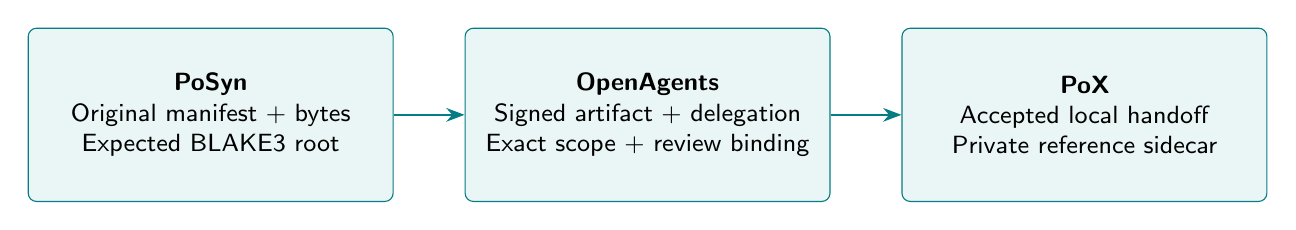
\begin{tikzpicture}[box/.style={draw=teal,fill=pale,rounded corners=3pt,text width=44mm,minimum height=22mm,align=center,font=\small\sffamily},arr/.style={-{Stealth},thick,draw=teal}]
\node[box] (p) {\textbf{PoSyn}\\Original manifest + bytes\\Expected BLAKE3 root};
\node[box,right=9mm of p] (o) {\textbf{OpenAgents}\\Signed artifact + delegation\\Exact scope + review binding};
\node[box,right=9mm of o] (x) {\textbf{PoX}\\Accepted local handoff\\Private reference sidecar};
\draw[arr] (p)--(o);\draw[arr] (o)--(x);
\end{tikzpicture}
\end{center}
{\footnotesize\color{grey}Figure 1. Implemented source boundaries: \texttt{chimiaclaw-posyn}, \texttt{chimiaclaw-federation}, and \texttt{integrations/pox}. Arrows denote local verification and reference exchange, not scientific execution.}

\sub{What the recipient can verify}
\begin{tabularx}{\textwidth}{@{}p{35mm}Y@{}}\toprule
\textbf{Evidence identity} & Original PoSyn manifest and object bytes; separately pinned root; strict file inventory, sizes and digests. Accepted, unsupported, rejected and missing records are transported unchanged.\\\addlinespace
\textbf{Signing authority} & Explicit public-key pins; separate human/AI identities; a producer's bounded AI delegation; local revoked-key and revoked-delegation lists.\\\addlinespace
\textbf{Review applicability} & Three distinct human roles, exact scope/handoff, exact evidence hash, designated reviewer signature and the retained review outcome.\\\addlinespace
\textbf{PoX relationship} & Existing staff authentication and accepted scope read through pinned source code. Fresh verification precedes a separate, append-only private reference record.\\\bottomrule
\end{tabularx}

\sub{A three-person handoff}
\begin{center}
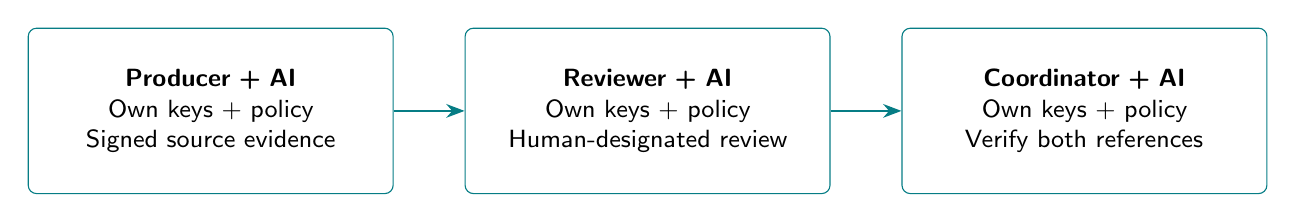
\begin{tikzpicture}[box/.style={draw=teal,rounded corners=3pt,text width=44mm,minimum height=21mm,align=center,font=\small\sffamily},arr/.style={-{Stealth},draw=teal,thick}]
\node[box] (a) {\textbf{Producer + AI}\\Own keys + policy\\Signed source evidence};
\node[box,right=9mm of a] (b) {\textbf{Reviewer + AI}\\Own keys + policy\\Human-designated review};
\node[box,right=9mm of b] (c) {\textbf{Coordinator + AI}\\Own keys + policy\\Verify both references};
\draw[arr] (a)--(b);\draw[arr] (b)--(c);
\end{tikzpicture}
\end{center}
{\footnotesize\color{grey}Figure 2. The executable demonstration uses three isolated directories and six fresh keys on one host. Only packages and public identity records cross these boundaries; this does not demonstrate OS-level isolation or three-device deployment.}

\callout{\textbf{Zero smart contracts required.} No new payment, custody, public registry, web endpoint or laboratory execution is introduced. The existing seven Solidity scaffolds are outside this exchange path.}

\newpage
\lead{02 / VERIFICATION AND USE}{Keep the claims\newline attached to the evidence.}
\callout{\textbf{Verified locally:} 167 Rust workspace tests; 10 real-source PoX
adapter tests; 27 three-installation exchange checks; 14 actual PoX/Rust journey
checks. The independent review found no remaining blocker for this offline pilot.}
The Rust total includes 10 PoSyn and 18 federation regressions. The new crates
pass scoped formatting and warning-denied Clippy. The PoX source tests use the
separately installed implementation; public CI runs five portable adapter tests
and explicitly skips those five source-dependent tests. A whole-workspace
formatting check still reports pre-existing differences in unrelated crates.


\sub{Trust is explicit and local}
Each participant creates their own key files, exchanges public keys through a
separately trusted channel, and pins the expected PoSyn root. Keys embedded in
received packages never enroll themselves. Policies include scope and expiry;
verification reports \texttt{local\_snapshot}, not universal current validity.
Remote revocations must be received before they can affect local decisions.

\textbf{Human-designated is not human presence.} The verifier rejects AI-designated
keys attempting a human review. An AI with the same operating-system access could
still read a human's plain key file. Keep review keys outside AI-accessible accounts
or signing environments. Hardware/user-presence signing is not implemented.

\textbf{Signed is not encrypted.} Private packages require a private transfer
channel. A recipient can retain delivered bytes; later revocation cannot erase
them. This tool offers no public-export or automatic-upload path.

\sub{What remains unestablished}
\begin{tabularx}{\textwidth}{@{}p{35mm}Y@{}}\toprule
\textbf{Scientific claims} & Execution remains \texttt{not\_verified}, reproducibility \texttt{not\_checked}, and physical synthesis \texttt{not\_attested}. A review signature does not establish scientific correctness.\\\addlinespace
\textbf{Delivery authority} & A PoX reference creates no source download capability, holder acceptance or release permission. Existing DFT delivery restrictions remain intact.\\\addlinespace
\textbf{Operations} & No hosted service, independent-device qualification, automatic trust synchronization, encrypted envelope, key recovery or hardware signing is delivered.\\\bottomrule
\end{tabularx}

\sub{Reproduce the public synthetic exchange}
\begin{quote}\ttfamily\small
cargo build --locked -p chimiaclaw-federation\\
python3 demo/federation/run.py
\end{quote}
The public fixture contains four wholly synthetic objects. The original PoSyn
verifier independently accepted its wire representation and expected root. The
real PoX demonstration additionally requires the separately installed, pinned
PoX source; it creates disposable synthetic inquiries and never opens a user's
existing database. See \path{integrations/pox/README.md} for that command.

\sub{Delivery evidence}
\path{VALIDATION.json} records exact checks and limitations;
\path{FEDERATION_DEMO.json} and \path{POX_DEMO.json} retain synthetic receipts.
Source identities and PDF inspection are recorded separately. Re-run verification
after any source change; a passing prior receipt is not evidence for edited code.
Publication and hosted-CI results are recorded in \path{PUBLICATION.json}
after the push. Branch: \path{integrate/posyn-pox-20261027}.
\end{document}
